\begin{savequote}[10cm] % this sets the width of the quote
\sffamily
The other thing I want to say is every dollar that is spent on the NDIS, you ordinary -- disabled and non-disabled -- Australians will see come back to your own pocket because all the NDIS does, it means a disabled person is able to get out of the house, go to the local shopping centre, buy themselves a coffee [\ldots] and they're going to spend that money in the community. 
This is not money that you're giving to disabled people that's going to go offshore into an offshore bank account earning interest somewhere. You are going to see every dollar of the NDIS come back to you because it's going to mean that disabled people are working, paying tax on their income, employing carers, carers pay tax on their income. [\dots] Every pound that England spends on access to work, which is similar, [\ldots], the economy receives £1.48 back. So it actually makes economic sense to give the disabled community access to these resources.
\qauthor{Kiruna Stamell}
\end{savequote}

\chapter{Health and Well--being}
\label{chap:health}

\section{Main Message}

Lives can be saved and quality of life significantly improved through the use of appropriate technology to lower the cost of health care, increase the speed of delivery and improve the quality of that care.

Australia has historically used technology such as radio, air transport and now satellite and internet based systems to counteract the disadvantages of living in remote areas. Technology can be shown to decrease the cost of delivery of health care, to improve the speed of delivery and to improve the quality of outcomes of that care. Technology is a key weapon in improving the efficiency and efficacy of health care delivery as health care, along with other professions such as education and the practice of law, is a service that is resistant to change. New technologies hold promise for solving key issues for disciplines where big data systems can achieve improvements in drug treatments and vaccines in years that would take traditional human processes decades. Technology has been seen as a panacea in Australia for a range of issues that contribute to poor health outcomes for non-urban Australians. Technologies such as the radio, telephone and finally satellite communications have been seen as ways of delivering expensive health services to non-urban clients in an affordable fashion. Proof of concepts have been shown to be successful again and again but there are important forces that moderate efforts to install new technologies in the health systems. Health, along with fields such as the Arts and Education exhibits a `cost disease' where it is difficult to automate processes as they are usually delivered by people to other people, reducing opportunities for IT process improvement. 
Australians in remote and very remote locations often have health outcomes that are worse than developing countries and Australia's performance on delivering health care to remote people has consistently failed to improve against the UN Millennial Development Goals and the Closing the Gap goals. There is some hope that networked systems being introduced and an emphasis on capacity building programs based around these networks will improve health care and make IT based health care delivery a reality for clients in these regions. Unfortunately, government and private companies are tending to move health support and delivery systems to IT and communications technology that is not always available or usable by remote and regional Australians. There is also a flip side to conquering `cost disease' that is known as `Jevon's Paradox' where, as a service becomes cheaper, consumers use more of it while still spending the same amount, negating the cost saving justification of installing and using the new technology. 

\section{The effect of technology on health}
Moore's law is driving improvement in research but ICT driven research currently outpaces Moore's law.
\begin{figure}
\centering
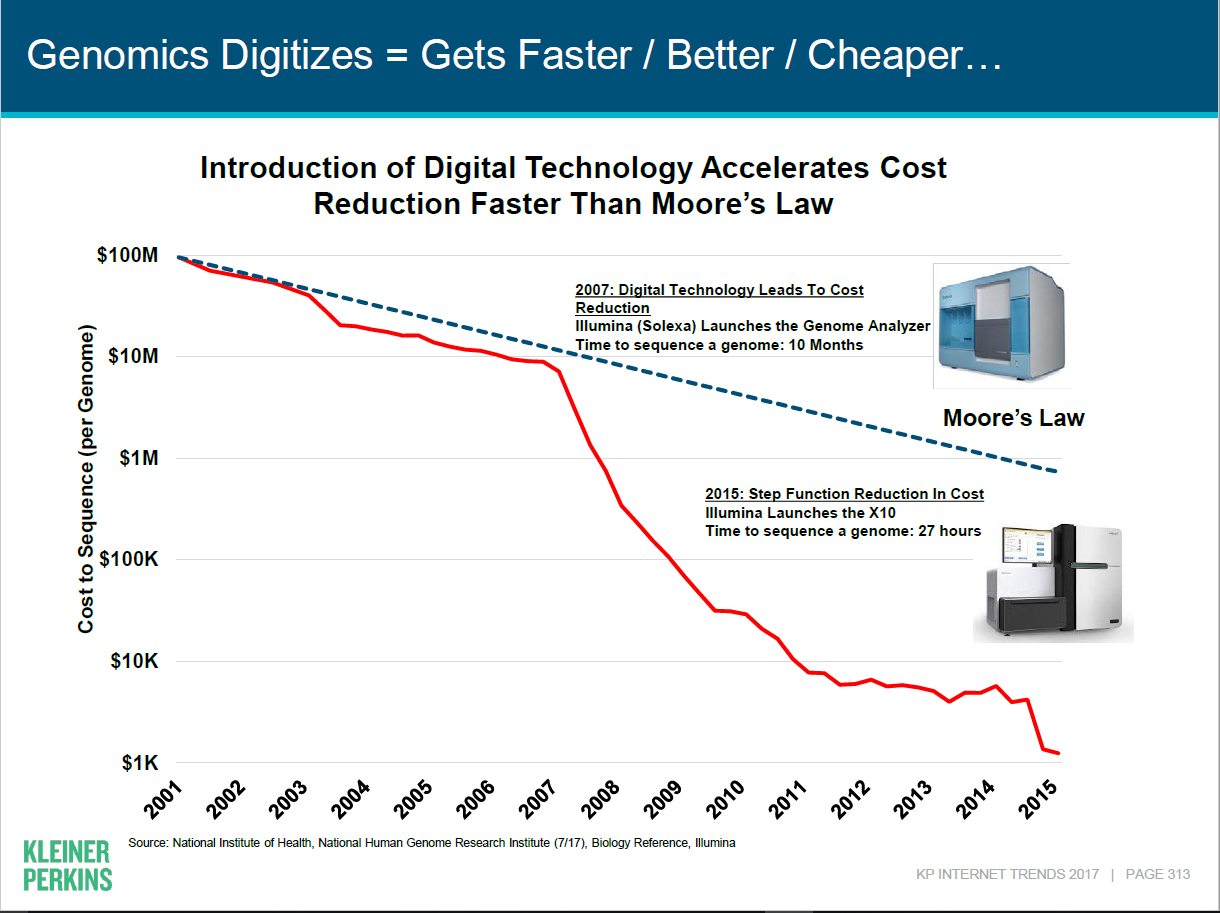
\includegraphics[scale=0.5]{figures/MaryMeeker2017-313GenomicsAndMooresLaw.png}
\caption{Digital Technology Accelerates Cost Reduction Faster Than Moore's Law\cite{RefWorks:249}}
\end{figure}
The cost of ICT continues to fall relative to other technologies and services.\cite{RefWorks:323} Advanced IT has never been cheaper or more easily deployed in remote communities. The cost of mobile computing devices in the form of smart phones and tablets falling below the cost of a tank of petrol or a basket of shopping and  available at post offices, stationary stores and supermarkets. It is tempting to believe that a ubiquitous, always on, ICT platform for health is already with us. It is possible to imagine that rural and remote health clients will be having online video conferences with their GP, sending their medical instrument telemetry via Bluetooth and monitoring eye and other chronic conditions via the NBN. When the NBN was first mooted this was the theory, as it had been the theory for every other communications technology beforehand. The Federal Government has commissioned \$20.3M worth of studies(4) to discover if this technology can be used to improve outcomes, reduce cost to serve clients and find a use for their new technology communications platform.

\section{Health Economics}
ICT enables the swift delivery of health advice to patients, sometimes without needing a health professional to deliver the information or recommendation. In the United States, more people visit WebMD, an online drug information and health advice site than visit a GP\cite{RefWorks:365}. This advice is free and replaces costly provision of health professionals. If people in remote areas cannot access the internet then they are doubly disadvantages since the only health advice they can get is from health professionals that they have to physically visit or telephone (if they have access to a telephone line). This consumes more time and has a greater than zero cost that is not present when using an system such as WebMD for a casual diagnosis or to check medication for side effects and dosages for medication they may already have.




\subsection{Cost disease in health}
ICT cannot improve productivity when that activity is based around what the economist, William Baumol called `stagnant service'\cite{RefWorks:322}. These are activities that have already been reduced to or are defined by the fixed amount of time they require to execute. A concert performer must still take the same amount of time to play a musical piece as when it was written a decade or a century ago as an example. Some biological processes, such as obstetric labour, have not kept pace with improved labour market productivity. We are reminded that `labour' implies an act of significant effort over time. As one journalist remarked,
\begin{quotation}
 In a world that moves at the speed of 140 characters, the former Kate Middleton offered a labor that, in contrast, proceeded at the pace of an Andy Warhol movie. How very inconvenient.

From the somehow simultaneously bored yet berserk coverage of the past few days, you'd get the impression that no one in the media had ever actually witnessed or experienced the time-consuming, complicated process of bringing a tiny human into the world.\ldots

On Fox News Monday morning, Martha MacCallum irritably noted that she'd been waiting ``about a week'' outside London's St. Mary's hospital but added the hope that Kate ``could be moving along quite quickly.'' She also nonsensically added that Princess Diana had labored for sixteen hours, speculating on ``whether or not that will have any impact on what we see here.'' (Hint: Why on earth would it?) CBS likewise impatiently reported that the ``Great Kate Wait'' was at last drawing to a close. ABC brought in an obstetric expert to answer George Stephanopoulos's exasperated question, ``How long is this gonna take?'' and ballpark, I kid you not, how efficiently the young prince might navigate the duchess' pelvis. And Huffington Post devoted a feature to ``what you have to budget for,'' timewise, for the thing to finally be over\cite{RefWorks:325}.
\end{quotation}    

Yet there are ways to take costs out of any process and health processes are no exception. While a consultation may take a standard 15 minutes, it is possible for nurse practitioners to perform many of the basic examination tasks of a general practioner (GP) and provide the GP with  a condensed summary of the patient's condition so that their expert examination technique is only required for those areas that are beyond the skills and training of the nurse practioner. Similarly, the rise of births by caesarian section means that ``[i]n the time it takes to assist a single natural birth, a medic might perform several Caesareans\cite{RefWorks:366}.'' Nonetheless, no amount of lean manufacturing style of performance improvement will reach the levels of increased productivity found in ICT systems that improve at an exponential Moore's Law rate


Since salaries continue to increase in line with inflation, the cost per unit of labour does not remain static but it increases. Many country's health systems are struggling with this phenomenon and how to fund increasingly expensive health care systems to deliver good patient health outcomes(12). ICT alone cannot change the cost of the stagnant services such as the cost of a surgeon's time in the operating theatre or the duration of a regular GP visit. It can remove travel time that takes place between appointments. Telehealth can deliver services through video conferencing and communications links and is providing a whole new market of patients who, until now, have been non-consumers of discretionary medical services because it takes too long or is too expensive for them to get to a health professional. 

\subsection{eHealth Systems}
eHealth systems, electronic interfaces designed to cut the time and expenses required for patient attendance, form filling and business process management are one ICT based solution to improve the process of health care delivery. Rather than paper based systems that require patients to fill out paper forms and for medical practitioners and their staff to reeneter this data, with possible errors, into anohter system, eHealth systems and can provide information to the service provider through fast information retrieval 

eHealth systems can also reduce problems associated with comorbidity and repeat diagnosis by providing an integrated patient record. Software in the doctor's patient mangement system can show recommended drugs and their side effects, treatments and other wellness information and can make referrals onto specialists that are contatined within its database; all without the practitioner having to refer to paper notes, card files, books or make telephone enquiries. This saves doctor and patient time but also improves the quality of the patient visit by providing more information that is more integrated than in a non-electronic environment. Patients can make appointments out of hours without having to wait to talk to a receptionist to find when their doctor is free. They can be connected to both Medicare, the Australian government's public health insurance agency but also to private insurance firms so that any payment can include the amounts that would be automatically refunded for the visit rather than the patient having to meet the full cost of the visit and submit several paper claim forms to the relevant agencies, wait for refund cheques and then wait for those checks to clear. This goes to the idea of electronic payments systems improving the velocity of money in the financial system. A payments cycle that would take several weeks using mail using paper is compressed to the speed of the transaction with eHealth system as the patient can even have their payment come out `just in time' at the doctor rather than having to have an indeterminate amount of cash on hand for a doctor visit.

The Australian government has spent over a billion dollars to implement a national Personally Controlled Electronic Health Record (PCEHR) to lower the cost of providing healthcare in this country. It will spend an additional \$374 million to update this system, which will now be called MyHealthRecord, to be an opt-out system rather than the opt-in system which has had a very poor adoption rate\cite{RefWorks:366}. Some reasons cited for introducing a PCEHR include reducing incorrect medication

\begin{quotation}
A financial incentive also exists for a well‐implemented and functioning system. On 10 May
2015, when announcing the PCEHR system overhaul and rebranding to My Health Record,
federal Minister for Health Sussan Ley stated `a fully-functioning national e-health system
could save taxpayers \$2.5 billion per year within a decade by reducing inefficiencies,
with an additional \$1.6 billion in annual savings also delivered to the states'. 
In a 2010 report by consultancy Booz \& Company, it estimated that fully digitising
the healthcare sector would realise \$7.6 billion in annual savings by 2020 and that this
figure only reflects direct savings and does not include savings through economic flow-on
effect.
\end{quotation} 

\begin{figure}
\centering
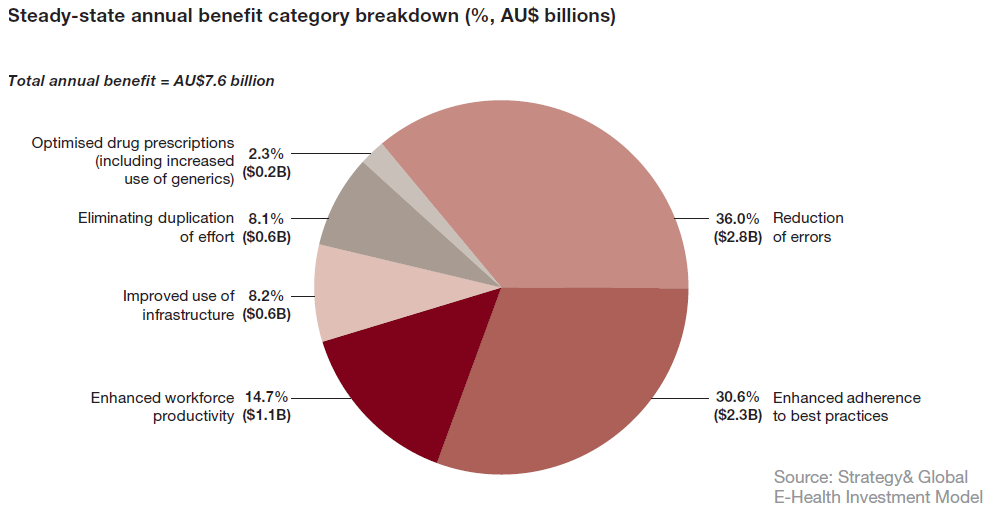
\includegraphics[scale=0.6]{figures/Optimising-e-health-value.png}
\caption{Economic value of Australian e-health in 2020 by benefit category\cite[p14]{RefWorks:368}}
\label{fig:SavingsEHealth}
\end{figure}

Although new treatments almost always cost more than the ones they replace, the affordability of those treatments seems to be falling internationally. This is due to two factors: ``A) The small, but positive, growth rate of productivity in the stagnant services and B) Productivity growth in the entire economy means we can afford more of everything\cite[p631-2]{RefWorks:208}.''

To point A, while health services are stagnant services, they are still influenced by inputs from other non-health systems that are experienceing, in some cases, substantial improvements in productivity such a that these stagnant systems do, over a period of time, improve slightly. They just do not improve at the rate of most of the services of the population. 

The point B, since the previously mentioned improvement in the cost of so many basic goods and services is decreasing, more of the average income is available for other services such as health and education.

\begin{figure}
\centering
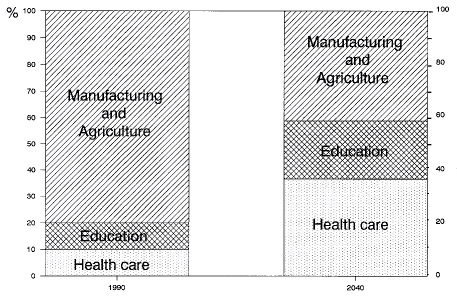
\includegraphics[scale=1.0]{figures/BaumolHealthSpendChng.png}
\caption{Hypothetical Changes in Total Spending, Over 50 Years, Assuming Historic Sectoral Productivity Growth Rates\cite[p633]{RefWorks:208}}
\end{figure}

It may be because everyone is using more and more IT to compress or eliminate the various tasks involved in the process
It may be due to superior treatments that are being developed, often with the aid of massive research projects driven by super computers that develop and simulate drugs such as immunosuppressants, anti-viral and anti-cancer drugs and therapies. Overall, the cost of disease in the community for many diseases is reduced by an order of magnitude or eliminated. Where once many women would have developed cervical cancer and men and women would have developed oral and rectal cancer due to HPV, the incidence rate of this disease is dropping off at dramatic levels due to a vaccination program for the HPV vaccine. Hepatitis, previously a death sentence through renal failure, is now treatable with a course of drugs lasting no more than a few weeks. The development of more advanced combinatorial therapies known as Pre-Exposure Prophylaxis (PrEP) has enabled HIV positive women to carry babies that are born HIV negative and for HIV positive or sero-discordant (where one parent is HIV positve and the other not) to conceive HIV negative children. Where previously these children would have had a lifetime of expensive therapies to look forward to, now they have no disease burden to live with.

It would be right to say pharmacology and other advances are responsible for these life saving advances but it would not have been possible to achieve such large--scale change on such complex problems if technology were not improving at the greater-than-Moore's Law speed.

Every chronic disease patient that can be removed from treatment is a potential saving of thousands or hundreds of thousands of dollars. If Australia's system was run along the same lines as the United States, every life saved by vaccination or treatment would be millions of dollars of costs that would not be added to the cost of health care.




\subsection{Jevon's paradox in health care}
As eHealth makes the delivery of health services cheaper, it does that mean that more services can be delivered for the same price. This does not tend to mean that the overall cost of healthcare falls, however, due to a phoneomenon first studied in the coal industry, Jevon's paradox. 



 
\subsection{Technology allows remote delivery of services}
Australia has a long history of delivering medical care over a distance. State health services are traditionally responsible for hospitals and medical care with some responsibility given over to the federal government as a consequence of World War II regulations. 
%reference required
These responsibilities have never returned to the states fully but there is a disparity between levels of care for health care recipeints in each state depending on the programs that are in operation there.

Services such as the Flying Doctor are the archtypical heavy capital style of health service delivery; the typical `ambulance at the bottom of the cliff instead of a fence at the edge of the cliff'.
%insert quote and pic
In times of crisis, remote and very remote health care users can call for the Flying Doctor and, if the local air strip is in good enough condition and the weather is good enough to permit it, it may be possible to send the air ambulance out to attend the patient for either medical evacuation to a regional facility or to be stabilised in their homestead or town. Even the Flying Doctor recognises that there are a lot of problems with this model of health care provision. It is expensive in terms of capital, the Flying Doctor have 66 planes but need more for peak times. Every year they manage over a quarter of a million patient contacts with over sixty-four thousand patient transports (an daily average of 177 transports). Telehealth has become an important treatment method with consultations outstripping the number of transport incidents (an average of 254 per day) with over ninety-two thousand telehealth consultations taking place in the 2014-2015 year. 

The Flying Doctor also operates a fleet of over 90 non--emergency road transport vehicles and has over twelve hundred staff devoted to its operations but they realise that sometimes the best way to deliver patient care is remotely. In a recent attempt to close the gap between patient survival rates in remote and very remote areas in South Australia and the urban centres.

\begin{quotation}
Heart Foundation evidence is that average death rates from coronary heart disease in men living in remote areas is 1.3 times higher than in city areas, and 1.2 times higher for women. A South Australian study of 29,623 episodes of myocardial infarction over a decade were assessed showing 30 day mortality was around a quarter higher in rural SA (705\/5,630 [12.52\%] compared to metropolitan SA (2,140\/23,993 [8.92\%]). Cardiologist-supported remote risk stratification, management and facilitated access to tertiary hospital-based early invasive management are associated with an improvement in 30-day mortality for patients who initially present to rural hospitals diagnosed with myocardial infarction. The interventions closed the gap in mortality between rural and metropolitan patients in South Australia.
\end{quotation}

Remote monitoring and patient care provided in tandem with video conferences over such low bandwidth solutions as skype, Apple Facetime or even fax
%reference heart study with faxes
have proved efficacious at diminishing illnesses from heart disease, eye care and most significantly, mental health.


%remember to note that health care in rural markets is uncontested

\subsection{Technology lowers Cost to Treat}
The commonly held view is that the cost to treat rural and remote patients is between five to seven times the cost to treat an urban patient. 
% citation required
This view ignores the fact that most of Australia is remote from urban centres and so the expected treatment mode for most parts of the country is remote treatment. The fact that most Australians live in an urban environment privileges a view that remote and rural users are expensive when it may be more productive, to view urban services as severely discounted due to the network effects of having facilities, specialists and resources required for health care in the same location as the patient. Over half a million people currently reside in rural and remote locations \cite[p7]{RefWorks:197} which makes this population larger than the population of the state capitals of both the Australian Capital Territory, Northern Territory and Tasmania and is around the same population of the City of the Gold Coast\cite{RefWorks:199} in Queensland but without it's own representative body at federal level. While it is the geographic responsibility of  many states, there are often differences in health and welfare outcomes to being in one state or another depending on access to health care programs and support services.
% insert comparative outcomes of health care in different states
Many treatment regimes require movement of the patient to the health care workers or specialist resources and facilities that are required to treat them in urban areas rather than treating the patient in place or, even better, looking at ways to prevent the diseases that afflict rural and remote Australians such as liver and kidney failure, chronic obesity, cancer therapy and treatment for accidental injury; all of which are the most common causes of illnesss in remote and very remote populations.


\subsection{Technology shrinks distance to Essential Services}

\begin{figure}
\centering
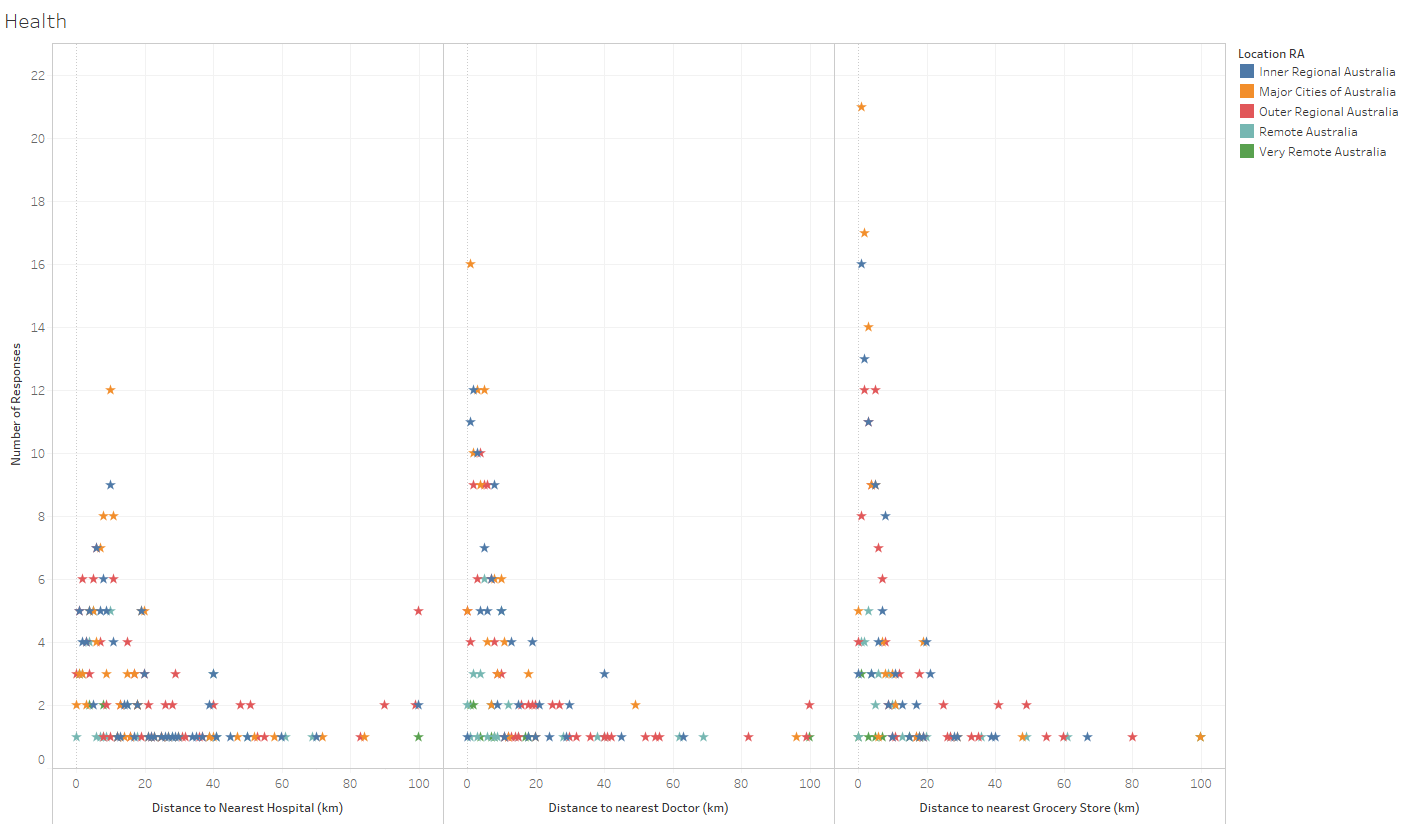
\includegraphics[scale=0.4]{figures/HealthDistances.png} 
\caption{Proximity to services by Region} \label{fig:VC05HospitalProxRegions}
\end{figure}
When framing questions on health care for my survey, I theorised that people in Remote and Very Remote Areas, even in Outer Regional Areas, might find accessing a hospital or doctor difficult due to their remoteness. Most respondents indicate that they live within 25 kilometres of a hospital which would indicate that, for the people doing this survey at least, a drive of several hours to access a high level of medical help is not required. I was also surprised to find that, even in Major Cities, some hospitals sometimes use video-conference systems to obtain access to a specialist outside of peak hours. When a relative broke his arm in the Blue Mountains and the hospital conducted a video-conference with another Sydney Hospital to obtain advice from an orthopaedic specialist\cite{RefWorks:371}. This saves having a specialist available at every Sydney Hospital every hour of the day but does point to the fact that hospital systems are taking steps to ensure they do not have expensive and scarce specialists waiting around on staff. It may be that, even when accessing a major hospital, patients might find that they are on a remote link with other specialists in different parts of a city, in another city or in another part of the world. 

\begin{figure}
\centering
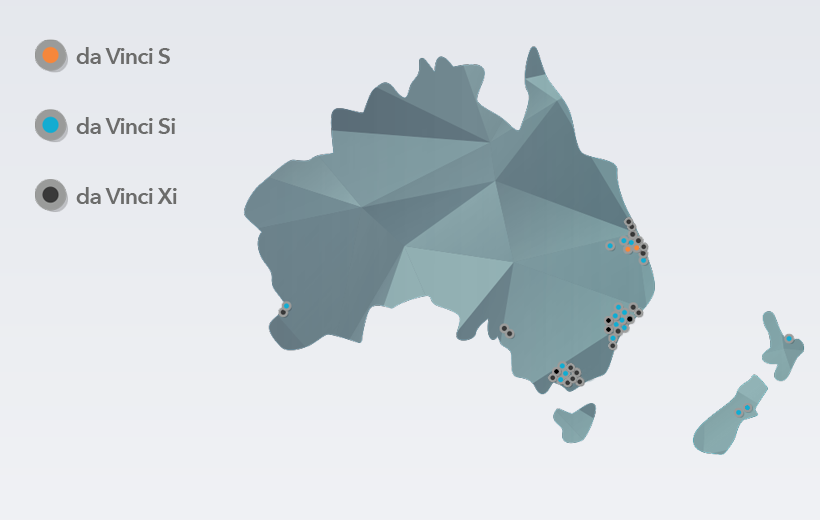
\includegraphics[scale=0.5]{figures/daVinciSurgery.png} 
\caption{Location of daVinci Surgery robots in Australia 2017\cite{RefWorks:374}} \label{fig:daVinciLocations}
\end{figure}
In this case, internet access for hospitals is definitely required and low latency access is required for robotic tele-surgery that is increasingly being performed where an international specialist can be engaged at a hospital in Australia to perform an operation without making the long trip to a an Australian hospital. While robotic surgery is now commonplace in many Australian capital city hospitals (see Figure \ref{fig:daVinciLocations}) there is a specific requirement to keep latency under control when performing robotic surgery. Surgeons typically perform their work at consoles removed from the patient in the operating room but it is possible to station the consoles several thousand kilometres away if the latency of the internet connection is under 200 milliseconds and, for an experienced surgeon, to compensate for delays of between 200 to 500 milliseconds. Above 500 milliseconds round trip time the delay is too great to risk robotic surgery. While all locations tested from Auckland to Moscow would suggest that it is possible to conduct this sort of surgery from any location in the world, in practice it is conducted in the same city at this point with only theoretical applications such as military hospitals in war zones being explored for international robotic surgery at this point\cite{RefWorks:373}.

While some respondents had to travel more than 20 kilometres to go to a hospital, almost all respondents had a doctor within 15 kilometres of their location(see Figure \ref{fig:VC05HospitalProxRegions}). Once again I theorised that in Remote and Very Remote Areas this would not be the case and that long journeys would be required for patients to visit their doctor. This may have come from the minority of doctors I had discussed the issue with at Broadband for the Bush conferences but it seems that almost all respondents are close enough to their local doctor to arrive there in under an hour by car.  

Even for those people, it may sometimes be preferable to order drugs over the internet when their doctor has provided a script. Outlets such as Discount Chemist Warehouse allow patients to mail their pharmacy script to them and the drugs are delivered by mail, often at a substantial discount and with an attendant time saving of not having to travel to the pharmacy to fill a script. For some medications that are provided as part of a trial such as the recent trial of a cure for Hepatitis C, or Pre-Exposure Prophylaxis (PrEP) are sometimes only obtainable using the internet to order the drugs from overseas sources. While the drugs may be declared safe for use and may be prescribed by an Australian doctor, because they are not listed on the Pharmaceutical Benefits Scheme, they must either be imported from overseas using websites such as Green Cross Pharmacy, All Day Chemist or AIDS Drugs Online or paid for a the local, unsubsidised price for the drugs from the manufacturer which can be 30 times the price or more. As an example, a month supply of PrEP, a drug that is used to prevent pregnant mothers with HIV giving the virus to their unborn children and to prevent the communication of HIV during unprotected sex, costs under \$40 a month from a supplier of the generic form of the drug while the brand name form of the drug would cost over \$840 for a month's supply.  In the case of the Hepatitis C drug, a twelve week supply of the drug Sofosbuvir retails for \$1,914.00 from the generic supplier Aids Drugs Online while the unsubsidised cost of the non-generic version of the drug obtained from the branded distributor has been, according to one study, as high as US\$94,500\cite{RefWorks:376}. It can be seen in these two cases that shopping over the internet is not merely a convenience, it can be a life-saving experience.



\subsection{Technology reduces travel costs}
\begin{quotation}
If, in the earlier parable, the hypothetical Mozart string quartet had been scored for a half-hour performance, then its performance in 1990 required two person-hours of labor, just as it did in 1790, when it might have been written. Thus, there is apparently no scope for the slightest increase in labor productivity. Yet that is only an illusion. To see why, assume that the more recent performance was by a Viennese group of musicians, and that it was played in Frankfurt am Main. A 1990 trip from their Austrian home base to the German auditorium surely would normally have taken no more than several hours. But when Mozart made the trip in 1790 it required six days of extreme discomfort (and, at that, Mozart wrote that he was surprised at the speed of the journey). Certainly, technical progress has reduced the number of hours of labor required to provide a unit of the output in question, thus raising the labor productivity of every itinerant performer, even in live performance (and we know that performers are virtually all itinerant).\cite{RefWorks:208}
\end{quotation}

\subsubsection{Technology makes trips less hazardous}
Residents of remote and very remote Australia are at a much greater risk of road death and injury than their urban counterparts. Public transport such as buses and trains are among the safest forms of transport but most trips in remote parts of Australia have to take place by car. These trips are often over poorly maintained roads or hazardous dirt tracks. Driving long distances induces fatigue and the desire to get to the end of the long trip faster may induce the driver to drive over the safe speed limit for the road. Driving under the influence is also more frequent in remote and regional areas where getting home from an event where alcohol was consumed by public transport is unlikely to be an option.

Vehicles are being improved with self driving technologies such as lane departure warnings that alert the driver by vibrating the steering wheel or sounding an audible alarm if they start to drift outside their lane and possibly into oncoming traffic or the side of the road. Systems such as Active Cruise which maintains a safe distance from the car in front are important in situations where a fatigued driver may not realise they are speeding up behind another vehicle that is slowing down in front of them until it is too late for them to react.

These systems are important saftey features that have been available in luxury models from some manufacturers but, like reversing cameras and ABS, are becoming commonplace on all vehicle price points from some manufacturers. Where internet connectivity can help is by connecting these systems together with a satellite and camera or LIDAR (Light Detection and Ranging) positioning system that can accurately map the vehicle's position on the road and, more importantly, can learn from the experience of other vehicles and actively avoid dangerous potholes, obstacles and other unsafe features. Using the automatic steering function, downloaded via an `over the air' update, Tesla Model S vehicles reduced the accident rate by 40\%\cite{RefWorks:352} Tesla cars can also avoid potholes

\section{The current situation in rural communities}
 The image of rural living is one of bucolic 'life on the land' where all the locals are healthy, well fed, happy individuals who eat a variety of nutritious foods in a close knit social community. The statistics tell quite a different story. Rural Australians suffer from very poor health outcomes. In some cases, these outcomes are worse than refugees from war--zones or developing economies such as sub--Saharan Africa. Higher than normal rates of diseases such as glaucoma, trachoma damage vision\cite{RefWorks:197}.
 
 
\subsection{Ear Disease} 
Australia has Ear diseases such as otitis media contribute to poor learning outcomes\cite{williams2009impact}.  Ear infections if left untreated lead to chronic conditions in rural areas where knowledge and practice of basic hygiene is lacking due to access to primary care workers, required medication and a support system that prioritises treatment of a disease which is invisible  though often painful to the patient. Damage occurs in the inner ear and, if left untreated, leads to reduction or loss of hearing and perforation of the ear drum. Since ear diseases affect rural Australians from an early age, they have a disproportionate impact on learning outcomes leading to reduced ability to learn and remain focused in educational settings. This reduces cognitive ability and has an impact on social development, causing children to be denied access to a social network. In an urban setting, children with hearing loss would have the benefit of educators, speech pathologists, speech therapists and learning development specialists that are a rarer commodity in a rural setting. 

Telephone coordination of efforts to diagnose, treat and monitor ear disease is a simple first step to ensuring efficient division of effort to educate people on proper ear health and ensure any issues are treated as soon as possible and proper education about maintaining ear health given\cite{hill2008tackling}. Trials have shown that it is possible for a field health specialist to use mobile broadband connected laptops to coordinate hearing aid fittings, testing and adjustment with urban based specialists which greatly increases both the number of patients who can be attended to by these specialists and reduces the burden of the specialist travelling for many hours or days to see only a few patients\cite{pearce2009pilot}. Queensland Health has been conducting a multi-year program to prove the efficacy of telehealth in ear care in remote and regional Queensland\cite{elliott2010feasibility} and Earbus has been running similar trials in Western Australia\cite[p10]{brook2013analysing}. Diagnostic vans with equipment to take video scans of children's ears to detect signs of ear disease regularly visit remote and outer regional communities that may not have access to a health clinic. Health professionals perform examinations in these locations and upload the images and hearing test results to the health department using mobile broadband for specialists to diagnose and recommend treatment or follow-up visits\cite{SmithAnthonyC2012Amte}. It is possible to make the field equipment even less complex using smart phones with otoscopes (ear microscopes) attached to take measurements and smartphone compatible otoscopes are but this equipment requires trained health professionals to produce useful medical images for specialists to examine\cite{ShahMananUdayan2018ioCa}. Hearing tests can also be administered using commodity  smartphones and tablets allowing diagnostic information to be delivered to specialist health care providers without delay\cite{brook2013developing} and reducing the reliance on fragile expensive equipment that may not survive in the hot dusty environment of remote Australia.
%picture of otoscope and earbus if time

\subsection{Eye Disease}

There are several trials and implementations of ICT that specifically target remote and very remote Indigenous Communities. The CSIRO is running an Eye Health study and Indigenous clients have been on eHealth systems for over a decade\cite{RefWorks:209}. Eye health is particularly important to remote and regional Australia where over half of the very remote communities surveyed have endemic levels of blinding trachoma\cite{RefWorks:210}. Since eye health professionals do not reliably attend these populations, a telehealth alternative to physical consultations is preferable to the health outcome of no consultation at all\cite{RefWorks:211}.

\subsection{Nutrition}
Rural Australian's nutrition is likely to be neglected due to poor dietary practices, a lack of fresh produce and a relatively sedentary lifestyle.  Previously, poor access to transport networks meant that people in Rural settings needed to be self-sufficient in terms of nutrition. When the nearest general store might be several hours drive away, only the food that could be grown nearby, potentially in their own gardens or in the local area would be accessible. Modern life has changed our perception of locally grown and sourced food and made highly processed prepared food more desirable through advertising and a systematic deskilling of the domestic cooking and nutrition skills of ordinary people. During the Depression of the 1920s, when people in Sydney around the suburbs of Marrickville and Redfern could not afford to buy meat they were able to live off protein in the form of rabbits that they caught in the local environment. The local football team in Redfern retains the name `Rabbitohs' as a reminder of its humble beginnings. In the period before reliable refrigerated road transport allowed logistics companies to extend supply chains deep into the regional and remote areas of Australia, locally produced food was all that was available. Now, in addition to providing such delicacies as Tasmanian salmon and seafood marinara mix hundreds of kilometres from the nearest ocean, fresh vegetables and fruit are road freighted into regional and remote areas where supermarkets have established a beachhead in the form of one of their stores.

These stores from supermarkets can serve the same function as the local community store, dispensing petrol, banking services through self--service checkouts and even delivery services that use their logistics and distribution to deliver parcels\cite[p22]{KPMG2014}. Retailers encourage delivery at supermarkets because it reduces their cost to ship online purchases to customers and supermarkets and petrol stations benefit as consumers often make an impulse purchase when they visit the business to collect their delivery\cite{FMCG2017}.

Remote and very remote areas do not have the number of customers that would be necessary to support the heavy capital investment of a supermarket and these areas still retain a local store function where people may have to drive several hours to purchase food and perform administrative functions. People in these remote and very remote areas may find themselves poorly served for fresh fruit, vegetables and meat with the preference given to items that have been heavily processed to increase their shelf--life. Studies (Voss) have used store purchase behaviour to show that nutrition, especially in remote and very remote areas, is often neglected and government and community programs have concentrated on improving nutrition in the diets of remote and very remote residents to improve health outcomes in those areas.

The internet has a role to play in being a conduit for community messages about healthy eating and making sensible purchasing choices. In the absence of other advertising, online ads sent to remote and very remote communities by government and community programs urging people to make nutritious choices have been shown to have an impact on purchasing behaviour [new zealand study on changing Indigenous eating practices]. Some communities have created apps to help residents and visitors understand locally sourced produce, `bush tucker',  can be eaten and how to prepare it, taking the place of traditional education that may have fallen out of use in some areas.

Healthy eating apps and exercise apps also have a role to play in improving diet and these work best with a reliable internet connection. Apps such as Fitbit or MapMyFitness can show healthy eating data such as the amount of fibre, carbohydrates, salt and fat in foods and in concert with a healthy eating program or a doctors advice can improve health outcomes for remote and very remote people who have been shown to be at greater risk of heart disease that is exacerbated by a high fat, high salt diet and from diabetes that is exacerbated by a high cabohydrate, high sugar diet. Many of these apps now allow the user to look up food by its barcode if it is one of prepackaged, manufactured items that is purchased in a supermarket and get a comprehensive analysis of the food as a meal and a breakdown of its properties. Once again, these apps work best if they are connected to the internet.
\begin{figure}
\centering
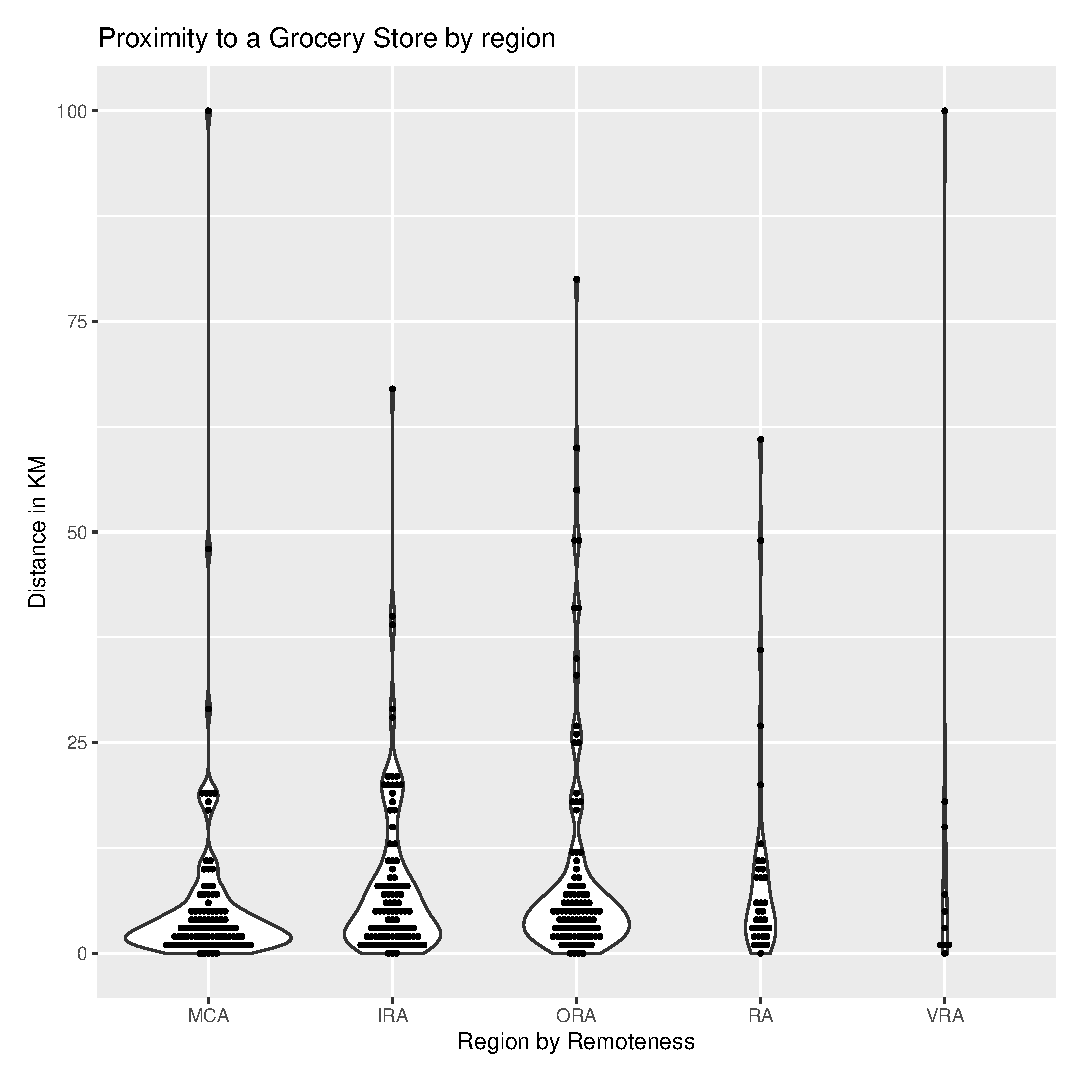
\includegraphics[scale=0.5]{figures/VChart09-Proximity2GroceryStore.eps}
\caption{Proximity to Grocery Store by Region} \label{fig:VC09GroceryStoreprox}
\end{figure}

In my survey I asked how far the respondent was from the nearest grocery store(Figure \ref{fig:VC09GroceryStoreprox}) to ascertain whether people in remote areas were more likely to drive long distances to acquire groceries. As a child, my family used to drive 40km to get decent fresh produce even though we lived in a farming area and were surrounded on all sides by diary farms, wheat fields and vegetable gardens. Surprisingly, very few respondents in each category reported travelling more than 15km for their groceries although inner and outer regional area respondents did travel further than major city respondents. Inner regional area respondents reported driving up to 25km in some cases to get to a grocery store but this may have simply been the distance from a small centre to the nearest large town. 


This question was primarily focussed on whether people in non-urban areas have good food security. Overseas experience has been that internet ordering through services such as Amazon Prime has seen the costs of many staples that are expensive at local grocery stores cut due to these services having free shipping options. The attraction of the Prime `shopping club' is that delivery on internet ordered items is free and also that shipping is guaranteed to be within two days of order. Amazon has indicated it will be starting a similar service in Australia but that it is currently hampered by poor delivery infrastructure for non-urban areas. While it is possible to deliver from a warehouse in Sydney to an address in Broome on the same day via air freight, for example, a current `air freighted' package would usually be flown to Perth from Sydney and then sent by road to Broome, taking between three and five days. A country where Amazon faces similar challenges is China where they currently offer Prime service but with a 5--9 day delivery time-frame.\cite{RefWorks:398}

These time-frames, which are typical of the challenges facing deliveries to regional locations, mean that shipping fresh produce is currently out of reach of internet delivery services and they are mostly confined to major cities. Amazon has had similar difficulties attempting to roll-out their fresh produce delivery service in North America and are investing in their own internal logistics network to overcome a reliance on the existing mail and freight delivery services.\cite{RefWorks:399} Although Amazon may be remaking worldwide logistics for internet deliveries in countries such as the US, China and Europe, there are large incumbents who can be expected to respond by either competing or, as Toll and Australia Post have indicated, working with Amazon on what is expected to be a AUD4Billion annual business\cite{RefWorks:400}.

\subsection{Remote Health monitoring}
An essential element of being able to treat patients in place and in diagnosing illnesses that may not always be expressed during a GP examination is taking repeated readings at intervals from patients over an extended period of time. Rather than travelling to a hospital or testing facility for an electro cardiogram, it may be both more revealing and be less strenuous to have the patient wear a heart monitor for a day or two and have the results sent back to a heart specialist for analysis. Rather than taking single blood glucose reading, it is possible to have the patient wear a glucose monitor and rather than having patients come into a sleep laboratory to check their sleep apnoea symptoms, they can obtain a remote monitor from a local chemist and have the results of their self administered test delivered to their specialist for a diagnosis\cite{ResMed2018}. 

%notes on fittness trackers for remote health monitoring


\subsection{Mental Health}
Although there is little traffic in remote and regional Australia, rural Australians are dependent on using the road network to access almost any service given the larger distance between them and service points. Rural Australians are also more likely to suffer from mental illness and commit suicide. A rural person has more than twice the chance of dying from suicide than they do from the previous largest cause of death, road accidents. 

\subsection{Suicide rate in non--urban communities}
\begin{quotation}
A study which sought to quantify the economic cost of suicide in Australia in 2012 estimated
the cost at A\$1.7 billion. This figure comprised direct costs related to coronial
inquiries, police and ambulance services, and counselling and support provided to family and
friends, and indirect costs, such as the lost economic contribution of an individual due to
premature mortality. The researchers demonstrated that 90\% of the economic
cost of suicide was attributable to male suicide due to the increased number of suicides by
males, the younger average age for male suicide (40.5 years) compared to female suicide
(44.3 years) and the higher income and employment rates for males.

\ldots

Farmers, young men, older people, and Indigenous Australians in remote areas are at greatest
risk of completing suicide. In 2010--2011, residents in very remote areas were almost twice as likely as those in major cities to die from
suicide. In 2015, residents living outside greater capital cities (16.2 deaths per 100,000 population) were 1.5 times as likely as residents of capital cities (10.8 deaths per 100,000 population) to die from suicide.
Residents of the Northern Territory (NT) (19.4 deaths per 100,000 population) recorded the
highest rate of deaths from suicide of all Australians.
This metropolitan-rural-remote differential was also identified by Cheung et al. who
conducted a spatial analysis of suicide mortality in Australia. The researchers found that males in
remote and rural areas demonstrated higher rates of suicide than males in major cities, and that
the rate of suicide amongst males increased with increasing remoteness.
In contrast to the pattern for men, the overall differences in suicide rates for females in remote
and rural areas compared to those in major cities, were not significant.
Between 2001 and 2011 suicide rates were consistently higher in all remoteness areas
compared with major cities. The greatest difference in suicide rates was observed
between very remote areas and major cities---suicide rates in remote areas were generally
between two and three times higher than suicide rates in major cities between 2001 and 2011\cite[p25-26]{RefWorks:326}.
\end{quotation}

\begin{figure}
\centering
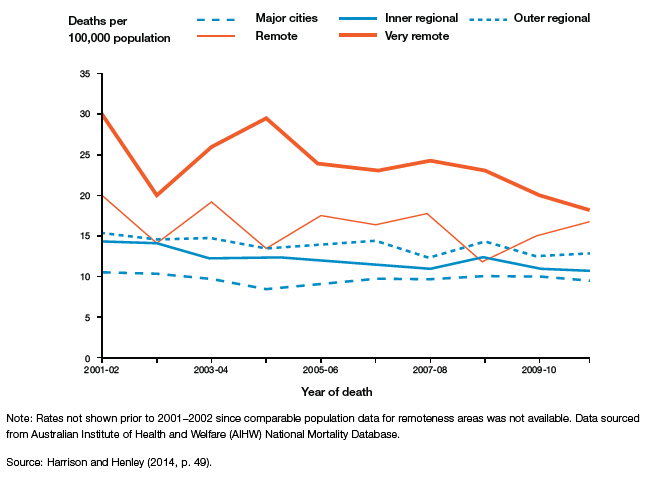
\includegraphics[scale=0.8]{figures/SuicideRatesRemoteCommunities.png}
\caption{Suicide rates, by remoteness area of residence, Australia 2001--2002 to 2010--2011\cite[p27]{RefWorks:326}}
\end{figure}


Anything that can reduce feelings of disconnection, lonliness and improve support for people living in remote areas would be a positive step to reducing. There is evidence that the rate of suicide is decreasing in urban areas but is continuing to rise in rural and remote areas, especially for young men\cite{Conv2012}. A possible reason for this might be that young men are moving to new oppotunities in urban areas and those who are still in remote and rural areas find themselves increasingly disadvantaged in terms of opportunities for work, standard of living and emotional connection where there are fewer suitible relationship options for them\cite{PitmanAlexandra2012Siym}. There is a lack of current information on trends in mental health in remote and rural areas and information predates recent installation of mobile phone and NBN networks in those areas so it is difficult at this time to know if better access to communications technology and social media is having a positive effect on the mental health of the non-urban population. 
